\part{Intro}
\chapter{Introduktion}
\label{chapter:introduktion}
Dette dokument er en samlet ressource til dokumentation af de netværksopgaver, der er udført med henblik på konfiguration og styring af automatiseringssystemer ved hjælp af TIA Portal, Studio 5000, Universal Robots og ABB's robotteknologi. Målet med dokumentet er at skabe en overskuelig guide, som kan assistere teknikere, studerende og undervisere indenfor automatiseringsteknologi med at forstå og udføre netværksrelaterede opgaver på tværs af forskellige automatiseringssystemer.
\newline\newline
\noindent Rapporten er opdelt i to hoveddele: Ethernet-baserede netværk og bus-baserede netværk. I TIA Portal-sektionen vil vi gennemgå opsætningen af kommunikationsnetværk for Siemens automatiseringshardware, hvilket inkluderer konfiguration af PROFINET. I Studio 5000-afsnittet vil fokus være på integrationen af Allen-Bradley udstyr og hvordan man opsætter Ethernet/IP netværk til industriel automatisering. For Universal Robots vil dokumentationen dække opsætningen af netværksforbindelser til UR-robotter, herunder fjernstyring og scriptkommunikation. Endelig vil ABB-robotafsnittet give vejledning i konfiguration af netværksparametre for ABB's robotter, med særlig opmærksomhed på RobotStudio.
\newline\newline
\noindent Hver sektion vil indeholde skridt-for-skridt vejledning, eksempler på konfigurationsfiler og fejlfindingstips for at sikre, at læseren kan navigere i opgaverne med tillid. Dokumentet er tænkt som en levende ressource, der kan opdateres og udvides, efterhånden som teknologierne udvikler sig og flere erfaringer bliver indarbejdet.

\section{Historie}
\label{section:historie}
For at forstå den nuværende tilstand og fremtidige retning for industrielle netværk, er det nyttigt at se på deres historiske udvikling. Her er nogle nøglepunkter i denne udvikling:

\subsection{Tidlige Systemer}
Før udbredelsen af digitale netværk blev industrielle systemer typisk styret af enkeltstående kontrolenheder og analog kommunikation. Dette resulterede i begrænset funktionalitet og fleksibilitet.

\subsection{Fremkomsten af PLC'er}
Programmable Logic Controllers (PLC'er) blev introduceret i 1960'erne og 1970'erne som en måde at automatisere og styre industrielle processer mere effektivt. PLC'er banede vejen for mere komplekse og fleksible automatiseringsløsninger.

\subsection{Serielle Protokoller}
I 1980'erne begyndte brugen af serielle kommunikationsprotokoller som RS232, RS422 og RS485 at blive almindelig i industrielle netværk, hvilket muliggør mere pålidelig dataoverførsel mellem enheder.
\newline\newline\noindent\textbf{RS232, RS422, RS485:} Disse er blandt de tidligste standarder for seriel kommunikation, introduceret i henholdsvis 1960'erne og 1970'erne. RS232 var en af de første bredt anvendte kommunikationsstandarder, der tillod forbindelse mellem computere og modemmer. RS422 og RS485 blev udviklet som forbedringer til RS232, hvor de tilbyder længere kabellængder og understøtter flere enheder på samme netværk. Disse standarder blev grundlaget for mange tidlige automatiseringssystemer.

\subsection{Fieldbus Teknologier}
I 1990'erne blev Fieldbus-protokoller som Profibus og DeviceNet udviklet, hvilket gjorde det muligt at forbinde mange enheder på et enkelt netværk med mere komplekse kommunikationsbehov.
\newline\newline\noindent\textbf{PROFIBUS (Process Field Bus):} Introduceret i 1980'erne, er PROFIBUS en af de tidligste standarder for feltbus kommunikation i industriel automatisering. Den blev udviklet for at standardisere kommunikationen mellem kontrolsystemer og feltudstyr, som f.eks. sensorer og aktuatorer. PROFIBUS understøtter både diskret og procesautomatisering og har været en af de mest udbredte industrielle netværksstandarder.
\newline\newline\noindent\textbf{DeviceNet:} DeviceNet, udviklet i 1990'erne, er baseret på CAN (Controller Area Network) og tilbyder en netværksløsning, der især fokuserer på lav-niveau enhedsforbindelser, såsom sensorer og aktuatorer. Den understreger enkelthed og omkostningseffektivitet i automatiseringssystemer.
\newline\newline\noindent\textbf{AS-I Bus (Actuator Sensor Interface):} AS-I Bus, introduceret i begyndelsen af 1990'erne, er designet som en simpel og omkostningseffektiv løsning til forbindelse af binære sensorer og aktuatorer. Det giver en nem måde at implementere en sensor/aktuator-niveau netværksinfrastruktur.

\section{Ethernet-baserede Netværk}
I slutningen af 1990'erne og begyndelsen af 2000'erne blev Ethernet-baserede netværk som Ethernet/IP og Profinet introduceret. Disse teknologier udnyttede de høje hastigheder og standardiserede kommunikationsprotokoller fra IT-verdenen og tilpassede dem til industrielle behov.
\newline\newline\noindent
\textbf{PROFINET:} Som opfølgeren til PROFIBUS, introduceret i begyndelsen af 2000'erne, er PROFINET en industriel Ethernet-standard designet til at imødekomme behovet for højere datahastigheder og realtid kommunikation. PROFINET udnytter standard Ethernet-teknologi og er optimeret til industrielle applikationer, hvilket giver større fleksibilitet og ydeevne.
\newline\newline\noindent
\textbf{Ethernet/IP:} Ethernet/IP, indført i slutningen af 1990'erne, er en industriel netværksstandard, der kombinerer traditionel Ethernet-teknologi med industriel protokol (CIP - Common Industrial Protocol). Den tilbyder en omfattende kommunikationsløsning, der understøtter både diskret og procesautomatisering.
\newline\newline\noindent
\textbf{Modbus RTU og TCP:} Modbus, udviklet i slutningen af 1970'erne af Modicon (nu Schneider Electric), er en af de ældste og mest udbredte kommunikationsprotokoller i industrien. Modbus RTU (Remote Terminal Unit) er en seriel kommunikationsprotokol, der anvender RS485 standarden, mens Modbus TCP/IP er en version af Modbus, der bruger Ethernet til kommunikation, hvilket gør det muligt at anvende standard netværksinfrastruktur til industriel kommunikation.
\begin{figure}[!h]
	\centering
	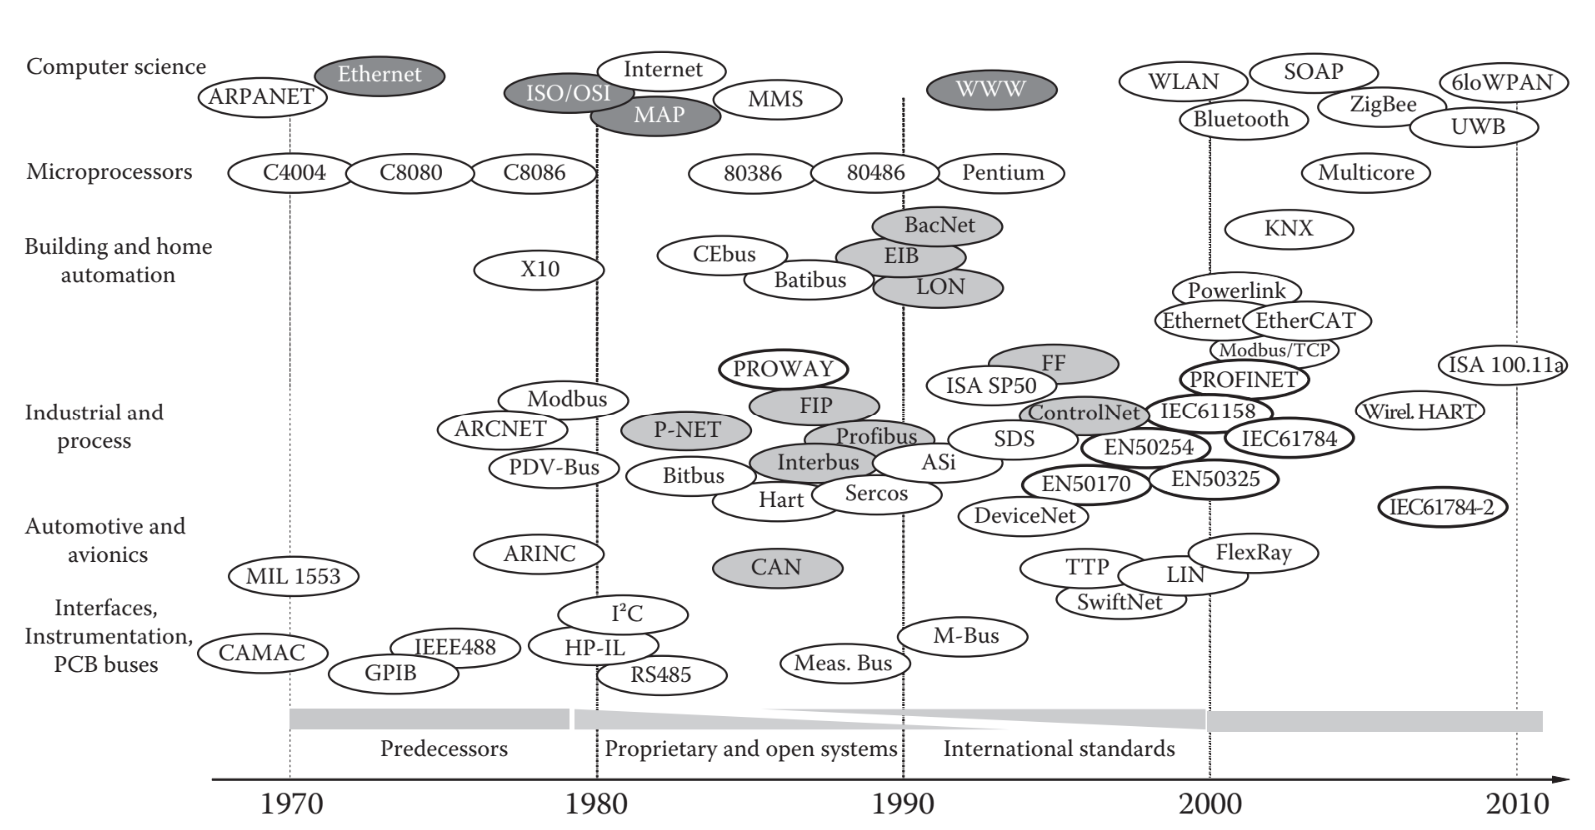
\includegraphics[width=\textwidth]{fig/fig32}
	\caption{Historisk visning af protokoller og standarder}
\end{figure}

\section{Industri 4.0 og IoT}
I det sidste årti har fremkomsten af Industri 4.0 og Internet of Things (IoT) revolutioneret industrielle netværk ved at integrere avancerede sensorer, cloud computing og big data-analyse, hvilket fører til mere intelligente og forbundne produktionssystemer.
\newline\newline\noindent
\textbf{IO-Link:} IO-Link, som blev standardiseret i 2006, er en punkt-til-punkt kommunikationsteknologi, der anvendes til at forbinde intelligente sensorer og aktuatorer til et automatiseringssystem. IO-Link er designet til at overføre både procesdata og diagnostiske data og giver mulighed for detaljeret sensor- og aktuatorstyring.
\clearpage